\subsubsection{simulate} \label{sec:simulate}

The operation \texttt{simulate} simulates a dynamical system and returns a trajectory starting from the initial state $x_0 = x(t_0) \in \Rn$ for an input signal $u(t) \in \R^m$ and a parameter value $p \in \R^p$. The syntax is as follows:
\begin{equation*}
	\begin{split}
		& [\texttt{t},\texttt{x}] = \texttt{simulate}(\texttt{sys},\texttt{params}), \\
		& [\texttt{t},\texttt{x},\texttt{ind}] = \texttt{simulate}(\texttt{sys},\texttt{params},\texttt{options}), \\
		& [\texttt{t},\texttt{x},\texttt{ind},\texttt{y}] = \texttt{simulate}(\texttt{sys},\texttt{params},\texttt{options}),
	\end{split}
\end{equation*} 
with the input arguments
\begin{center}
\renewcommand{\arraystretch}{1.3}
\begin{tabular}[t]{l p{13cm} }
	$\bullet$~\texttt{sys} &  dynamic system defined by one of the classes in \cref{sec:continuousDynamics,sec:hybridDynamics}, e.g., \texttt{linearSys}, \texttt{hybridAutomaton}, etc. \\
	$\bullet$~\texttt{params} & struct containing the parameter for the simulation \\
	 & \begin{tabular}[t]{l p{10cm}}	
	 	--~\texttt{.tStart} & initial time $t_0$ (default value 0) \\
	 	--~\texttt{.tFinal} & final time $t_f$ \\ 	
	 	--~\texttt{.x0} & initial point $x_0$ \\
	 	--~\texttt{.u} & piecewise-constant input signal $u(t)$ specified as a matrix for which the number of rows is identical to the number of system inputs \\
	 	--~\texttt{.p} & parameter value $p$ (class \texttt{nonlinParamSys} only) \\
	 	--~\texttt{.w} & disturbance $w$ (classes \texttt{linearSys} and \texttt{linearSysDT} only) \\
	 	--~\texttt{.v} & sensor noise $v$ (classes \texttt{linearSys} and \texttt{linearSysDT} only) \\
	 	--~\texttt{.y0guess} & guess for a consistent initial algebraic state (class \texttt{nonlinDASys} only, see \cref{sec:reachDAEsys}). \\
	 	--~\texttt{.startLoc} & index of the initial location (class \texttt{hybridAutomaton} and \texttt{parallelHybridAutomaton} only) \\
	 	--~\texttt{.finalLoc} & index of the final location (class \texttt{hybridAutomaton} and \texttt{parallelHybridAutomaton} only)
	 	\end{tabular}	\\
	$\bullet$~\texttt{options} & simulation options for MATLAB's \texttt{ode45} function (see \url{https://de.mathworks.com/help/matlab/ref/ode45.html}).
\end{tabular}
\end{center}
and the output arguments
\begin{center}
\renewcommand{\arraystretch}{1.3}
\begin{tabular}[t]{l p{13cm} }
	$\bullet$~\texttt{t} & time points of the simulated trajectory \\
	$\bullet$~\texttt{x} & states of the simulated trajectory \\
	$\bullet$~\texttt{ind} & index of event function triggered by MATLAB's \texttt{ode45} function (see \url{https://de.mathworks.com/help/matlab/ref/ode45.html}) \\
	$\bullet$~\texttt{y} & output trajectory (classes \texttt{linearSys} and \texttt{linearSysDT} only)
\end{tabular}
\end{center}

Let us demonstrate the operation \texttt{simulate} by an example:

\begin{center}
\begin{minipage}[t]{0.45\textwidth}
	\vspace{10pt}
	\footnotesize
	% This file was created by matlab2tikz.
%
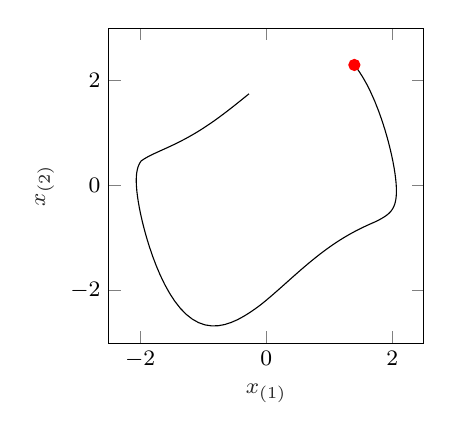
\begin{tikzpicture}
\footnotesize

\begin{axis}[%
width=4cm,
height=4cm,
at={(0in,0in)},
scale only axis,
xmin=-2.5,
xmax=2.5,
xlabel style={font=\color{white!15!black}},
xlabel={$x_{(1)}$},
ymin=-3,
ymax=3,
ylabel style={font=\color{white!15!black}},
ylabel={$x_{(2)}$},
axis background/.style={fill=white}
]
\addplot [color=black, forget plot]
  table[row sep=crcr]{%
1.4	2.3\\
1.4687	2.1884\\
1.534	2.0661\\
1.5956	1.9353\\
1.6532	1.798\\
1.721	1.6164\\
1.7819	1.4325\\
1.836	1.2504\\
1.8833	1.0735\\
1.9241	0.9049\\
1.9588	0.7464\\
1.9877	0.5995\\
2.0114	0.4648\\
2.0302	0.3424\\
2.0447	0.2322\\
2.0553	0.1334\\
2.0624	0.0455\\
2.0663	-0.0326\\
2.0675	-0.1018\\
2.0663	-0.163\\
2.0629	-0.2171\\
2.0576	-0.265\\
2.0506	-0.3074\\
2.0421	-0.3451\\
2.0323	-0.3787\\
2.0212	-0.4088\\
2.0091	-0.4359\\
1.9961	-0.4604\\
1.9821	-0.4827\\
1.9674	-0.5031\\
1.9519	-0.522\\
1.9358	-0.5396\\
1.919	-0.5561\\
1.9016	-0.5717\\
1.8836	-0.5866\\
1.8651	-0.6009\\
1.846	-0.6148\\
1.8265	-0.6284\\
1.8064	-0.6417\\
1.7859	-0.655\\
1.7648	-0.6681\\
1.746	-0.6797\\
1.7202	-0.6931\\
1.694	-0.7069\\
1.6672	-0.7211\\
1.6399	-0.7357\\
1.612	-0.7509\\
1.5836	-0.7666\\
1.5545	-0.783\\
1.5249	-0.8\\
1.4945	-0.8178\\
1.4635	-0.8365\\
1.4318	-0.856\\
1.3993	-0.8765\\
1.366	-0.898\\
1.3319	-0.9206\\
1.297	-0.9445\\
1.2611	-0.9696\\
1.2242	-0.9962\\
1.1864	-1.0242\\
1.1474	-1.0539\\
1.1073	-1.0853\\
1.066	-1.1186\\
1.0234	-1.1538\\
0.9794	-1.1913\\
0.934	-1.231\\
0.8871	-1.2732\\
0.8385	-1.3179\\
0.7882	-1.3654\\
0.736	-1.4159\\
0.6819	-1.4694\\
0.6258	-1.526\\
0.5675	-1.5859\\
0.5068	-1.6492\\
0.4437	-1.7159\\
0.3781	-1.7858\\
0.3097	-1.859\\
0.2386	-1.935\\
0.1646	-2.0136\\
0.0876	-2.094\\
0.0075	-2.1757\\
-0.0756	-2.2574\\
-0.0832	-2.2644\\
-0.087	-2.2678\\
-0.0908	-2.2713\\
-0.11	-2.2887\\
-0.1293	-2.306\\
-0.1488	-2.3231\\
-0.1684	-2.3402\\
-0.2613	-2.4172\\
-0.3571	-2.4887\\
-0.4554	-2.5524\\
-0.5559	-2.6053\\
-0.6581	-2.6447\\
-0.7615	-2.6674\\
-0.8654	-2.6707\\
-0.969	-2.6521\\
-1.0715	-2.6097\\
-1.172	-2.5426\\
-1.2694	-2.4508\\
-1.363	-2.3356\\
-1.4518	-2.1992\\
-1.5352	-2.0452\\
-1.6125	-1.8775\\
-1.6834	-1.7005\\
-1.7475	-1.5188\\
-1.8048	-1.3368\\
-1.8553	-1.1583\\
-1.8993	-0.9864\\
-1.9369	-0.8237\\
-1.9687	-0.6716\\
-1.9949	-0.5314\\
-2.0162	-0.4033\\
-2.0328	-0.2874\\
-2.0454	-0.1831\\
-2.0542	-0.09\\
-2.0597	-0.0071\\
-2.0624	0.0665\\
-2.0624	0.1317\\
-2.0601	0.1894\\
-2.0557	0.2404\\
-2.0496	0.2857\\
-2.0419	0.3258\\
-2.0327	0.3616\\
-2.0223	0.3935\\
-2.0138	0.4151\\
-2.0048	0.4351\\
-1.9952	0.4536\\
-1.9851	0.4709\\
-1.9595	0.4927\\
-1.9332	0.5131\\
-1.9061	0.5324\\
-1.8783	0.5509\\
-1.8498	0.5689\\
-1.8206	0.5864\\
-1.7908	0.6037\\
-1.7603	0.6208\\
-1.7292	0.638\\
-1.6975	0.6553\\
-1.6651	0.6729\\
-1.632	0.6908\\
-1.5982	0.7092\\
-1.5638	0.728\\
-1.5286	0.7475\\
-1.4927	0.7678\\
-1.456	0.7888\\
-1.4186	0.8107\\
-1.3802	0.8337\\
-1.341	0.8577\\
-1.3009	0.8829\\
-1.2598	0.9095\\
-1.2177	0.9374\\
-1.1745	0.9669\\
-1.1301	0.998\\
-1.0846	1.0309\\
-1.0378	1.0658\\
-0.9896	1.1027\\
-0.94	1.1418\\
-0.889	1.1832\\
-0.8363	1.2271\\
-0.7819	1.2736\\
-0.7257	1.3229\\
-0.6676	1.375\\
-0.6076	1.4302\\
-0.5453	1.4883\\
-0.4809	1.5495\\
-0.4141	1.6137\\
-0.3448	1.6808\\
-0.273	1.7505\\
};
\addplot [color=red, only marks, mark=*, mark options={solid, red}, forget plot]
  table[row sep=crcr]{%
1.4	2.3\\
};
\end{axis}
\end{tikzpicture}%
\end{minipage}
\begin{minipage}[t]{0.4\textwidth}
	\vspace{0pt}
	\centering
	\includetikz{./figures/tikz/contDynamics/example_simulate}
\end{minipage}
\end{center}
